\chapter{Tutorial to parallel BEAST/BEAGLE utility for sequence simulation ({\bussname})\label{app:pibuss_tuto}}
\chaptermark{Tutorial: {\bussname}}

\section{Introduction} 

The BEAST/BEAGLE utility for sequence simulation ({\bussname}) provides an easy to use interface that allows flexible and extensible phylogenetic data fabrication, delegating computationally intensive tasks to the BEAGLE library and thus making full use of multi-core architectures.
This document is intended as a guide through {\bussname}. The objective is to show the unexperienced user how to simulate character sequences (nucleotides, amino acids)  under a number of Markov models of evolution (HKY, GTR, TN93, GY94). Moreover, we show  how the user can set several partitions, with linked or unlinked parameters. All this can be achieved by using the friendly graphical user interface (GUI). {\bussname} also has a command-line interface (CLI), that allows for easy integration and pipelining, which may come in handy for big simulation studies. 
To gain access to the more advanced options and simulate under complex evolutionary scenarios users are encouraged to generate and edit XML files that can be then loaded into BEAST software.
All three interfaces will be presented in this tutorial.

{\bussname} is cross-platform and will run on Windows, Mac and Linux operating systems. It is implemented in java, and requires Java runtime environment version 1.5 or greater to run its executables. Also, the BEAGLE library needs to be installed. See \url{https://code.google.com/p/beagle-lib/w/list} for details on BEAGLE installation and use.

Windows users can run {\bussname} by opening a CMD and issuing:
 
\begin{code}
% java -Djava.library.path="C:$\backslash$Program Files (x86)$\backslash$Common Files$\backslash$ libhmsbeagle-1.0" -jar PATH$\backslash$TO$\backslash$buss.jar
java -Djava.library.path="C:$\backslash$Program Files (x86)$\backslash$Common Files$\backslash$ libhmsbeagle-1.0" -jar buss.jar
\end{code}
 
Note that this assumes BEAGLE is installed at the default location. If this is not the case, the user should supply the appropriate path for \texttt{Djava.library.path}. Also, mind the quotation marks, they are important.
% LM:  as a side note, if the BEAGLE installation went fine, you will not need to set the path to BEAGLE
% LM: don't have A CLUE on how to use a Mac :)
% FB: they also have terminals
% FB:  the goal is to ultimately have it all wrapped in a separate package for Win, Mac and Linux that detects BEAGLE, sets all the paths and then runs the software on double-click or with just one automated script

In a UNIX/Linux enviroment, the {\bussname} GUI can be called from the command line with

\begin{code}
java -Djava.library.path=/usr/local/lib -jar buss.jar 
\end{code}

\noindent
where \texttt{-Djava.library.path} again points to the directory where BEAGLE is installed.

\def\loading{Loading a tree topology}
\subsection{\loading}

In order to simulate character sequences, one will need a tree topology, with correspondent branch lengths, as  backbone. In {\bussname}, to import a tree, the user needs simply to go the \textbf{Trees} tab and click the `Choose file' button. After that, a window will open for you to browse though your files and go the desired tree file (see Figure~\ref{fig:loadingtopology}). {\bussname} accepts input trees in newick or nexus formats.

%%
\begin{figure}[h!]
\centering
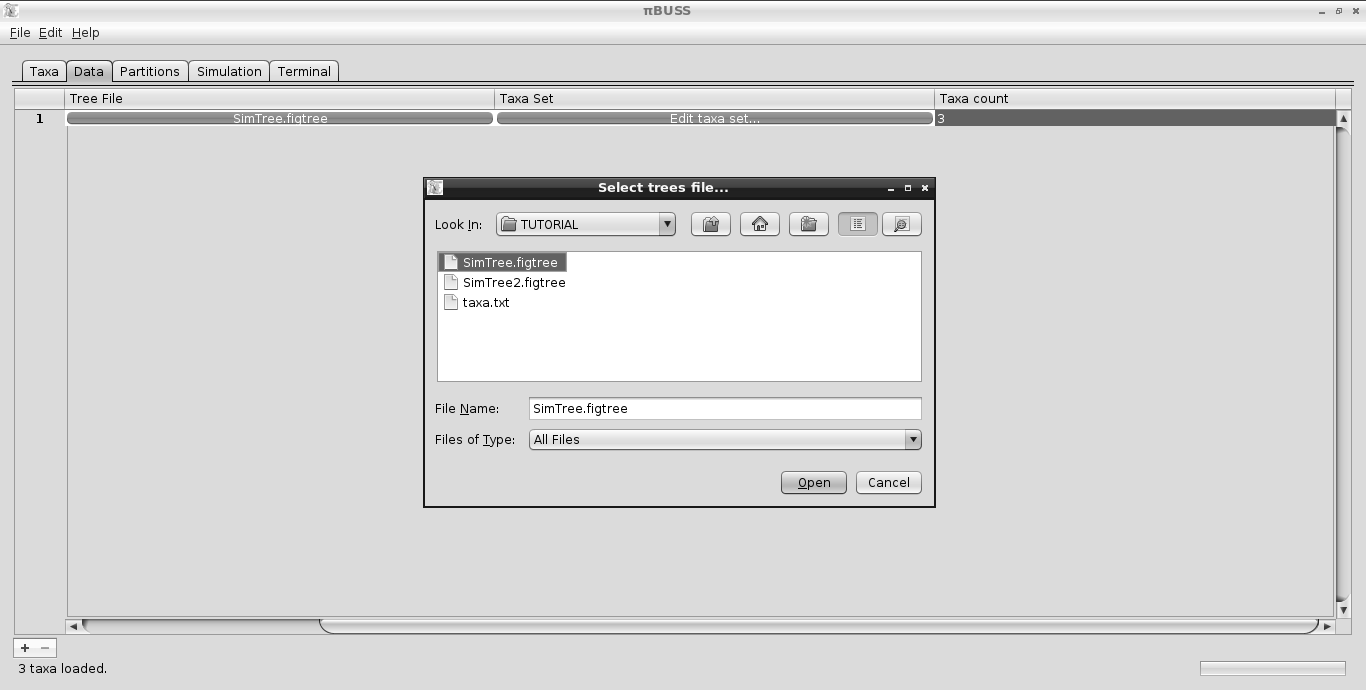
\includegraphics[scale=\figurescale]{LOAD_TREE.png} 
\caption{
{ \footnotesize 
{\bf How to load a tree into {\bussname}.}
} % END: footnotesize
}
\label{fig:loadingtopology}
\end{figure}
%%

After the tree topology is loaded, the user can check taxa names and branch lengths (tree heights) at the \textbf{Taxa} tab. 

\subsection{Setting a coalescent model}

The next step after loading a tree is to set a demographic coalescent model for the simulation. 
The default is to use the user-specified  tree. But sometimes one may be interested in simulating several demographic scenarios for a given set of taxa, and {\bussname} offers three such options. Currently, the user can choose between the Constant population and Exponential growth models, either by specifying growth rates or doubling times.% LM: will that be expanded in the future?

To select a demographic model for the simulation, the user needs to go to the \textbf{Partitions} tab and click  the \emph{Demographic model} button. 
Then she can choose between the three models and set the parameters. 
For \emph{Constant population} option, all that is needed is to set the population size parameter. 
For \emph{Exponential Growth}, the user needs to set both the population size parameter and a growth parameter, that can be either expressed as a growth rate or as doubling population times. 
Figure~\ref{fig:demographic} illustrates this step.

%%
\begin{figure}[h!]
\centering
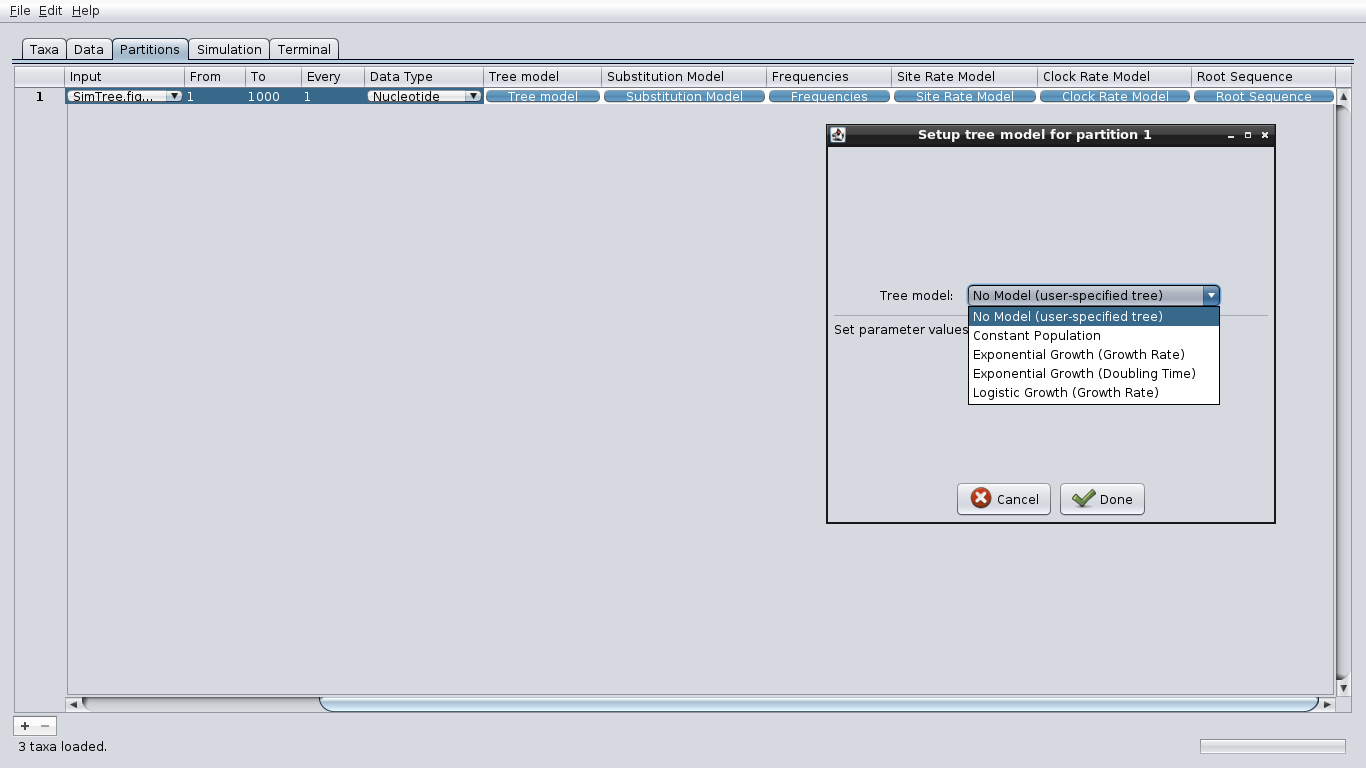
\includegraphics[scale=\figurescale]{DEMOGRAPHIC.png} 
\caption{
{ \footnotesize 
{\bf Choosing a demographic (coalescent) model.}
} % END: footnotesize
}
\label{fig:demographic}
\end{figure}
%%

\subsection{Branch substitution model}

After setting the demographic model, it is time to choose a branch substitution model, i.e., a Markov model of evolution. 
{\bussname} offers three models of nucleotide sequence evolution (HKY, TN93, GTR) as well as a codon model (GY94). 
Simulating data under models of different complexity is crucial to assess the accuracy of reconstruction methods and their robustness to model mispecification and asumption violation. 
Also, simulating data under a codon model allows generating data with known ratio of non-synonymous to synonymous mutations ($dN/dS$), which can in turn be used to test methods that try estimate this quantity and/or detect selection.
To choose a substitution model, go the \textbf{Partitions} tab, click the `Branch Substitution Model' and select the desired model. 
For each model, certain parameters have to be specified. 
For the HKY model, just the $\kappa$ (kappa) parameter needs to be set. 
For the TN93 model, the user needs to supply two $\kappa$ values, and for the GTR model, six base-transition parameters can be specified.
% New section on AA.

{\bussname} also offers the ability to simulate aminoacid sequences under several widely used empirical models, such as the BLOSUM62, Dayhoff, JTT, FLU and WAG. You can also specify your own aminoacid (base) frequencies by using the 'Base Frequecies' dropdown menu.  

%%
\begin{figure}[h!]
\centering
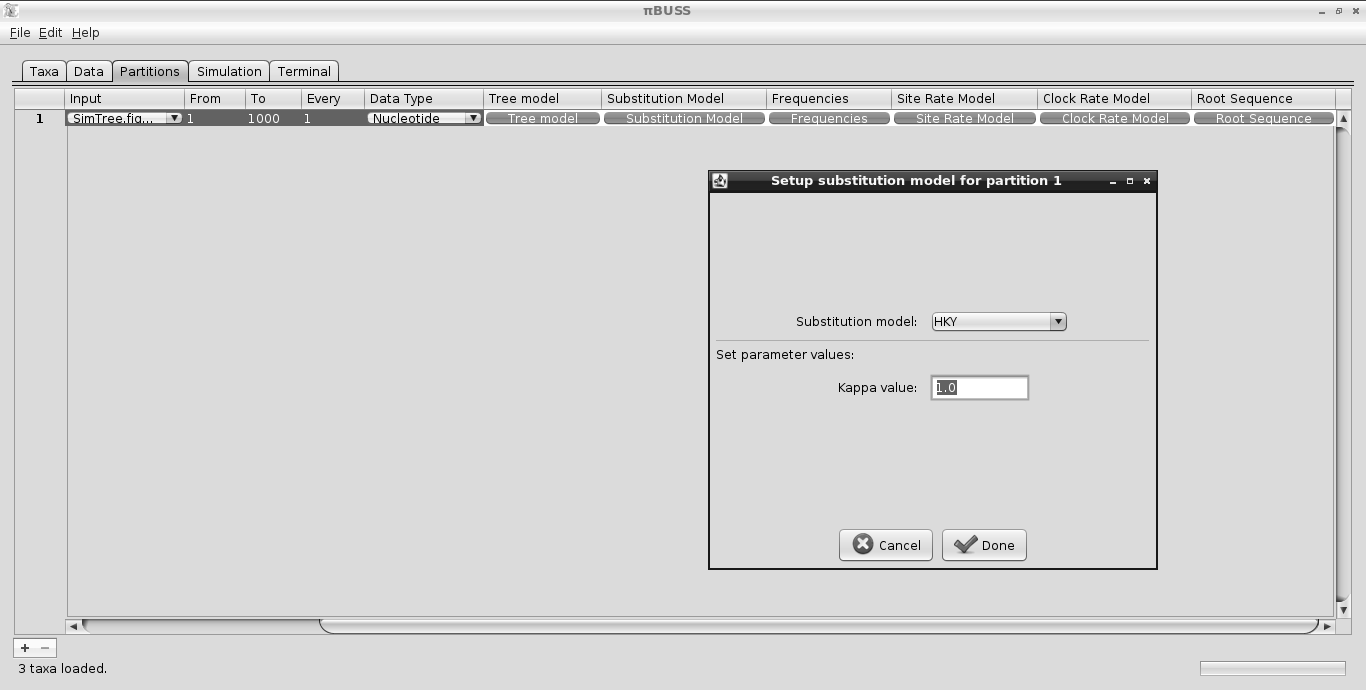
\includegraphics[scale=\figurescale]{HKY.png} 
\caption{
{ \footnotesize 
{\bf Setting a HKY substitution model with $\kappa$ parameter of $1.0$.}
} % END: footnotesize
}
\label{fig:hky}
\end{figure}
%%

The GY94 codon model takes two parameters, $\omega$ and $\kappa$. 
While $\omega$ (omega) controls the ratio of non-synonymous and synonymous substitution rates ($dN/dS$), $\kappa$ controls, as usual, the transition/transversion ratio. 
See Figures~\ref{fig:hky} and~\ref{fig:gy94} for examples.

%%
\begin{figure}[h!]
\centering
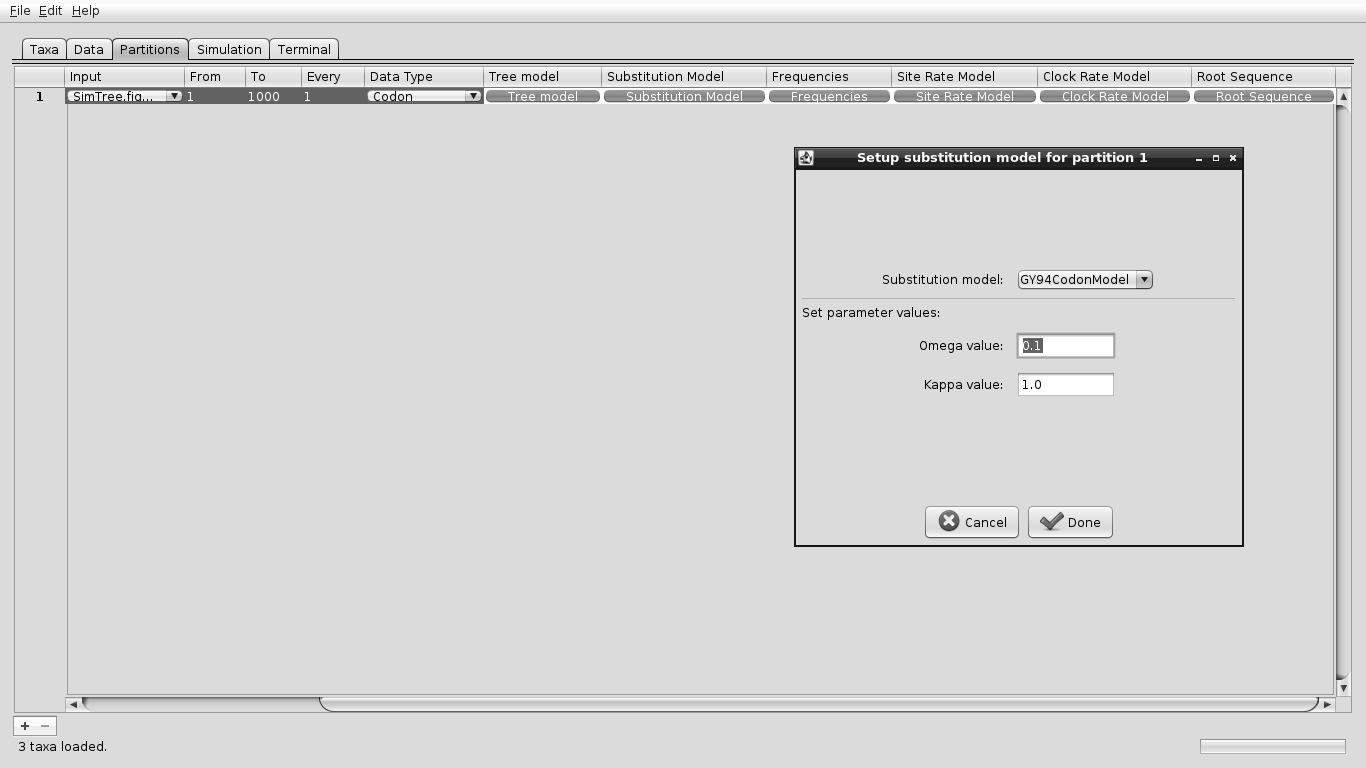
\includegraphics[scale=\figurescale]{GY94.png} 
\caption{
{ \footnotesize 
{\bf Setting a codon model (GY94) with $\kappa=1.0$ and $\omega=0.1$.}
} % END: footnotesize
}
\label{fig:gy94}
\end{figure}
%%

\subsection{Site Rate Heterogeinity and Base frequencies}

Classical models of evolution assume that that mutations are independent and identically distributed along a sequence. 
In the real world, however, this may not be case. 
Site rate heterogeinity is commonly modeled by assuming that mutation rates are distributed according to a discretized Gamma distribution.
The distribution is governed by two parameters: $\alpha$ and the number of rate categories. 
The $\alpha$ parameter controls how much heterogeinity is there between sites and the smaller the value of $\alpha$, the more dissimilar the rates between sites, with few sites having high rates and the rest being practically invariant.

Additionally, it may be appropriate to assume that a given proportion of the sites do not mutate at all, i.e., they are invariant. 
In {\bussname}, the user can add site rate heterogeinity to the simulated data by going to the \textbf{Partitions} tab and clicking the `Site Rate Model' button (Figure~\ref{fig:gamma}). 
There the user can specify how many categories should be created for the discretized Gamma distribution, as well as set the proportion of invariant sites.

%%
\begin{figure}[h!]
\centering
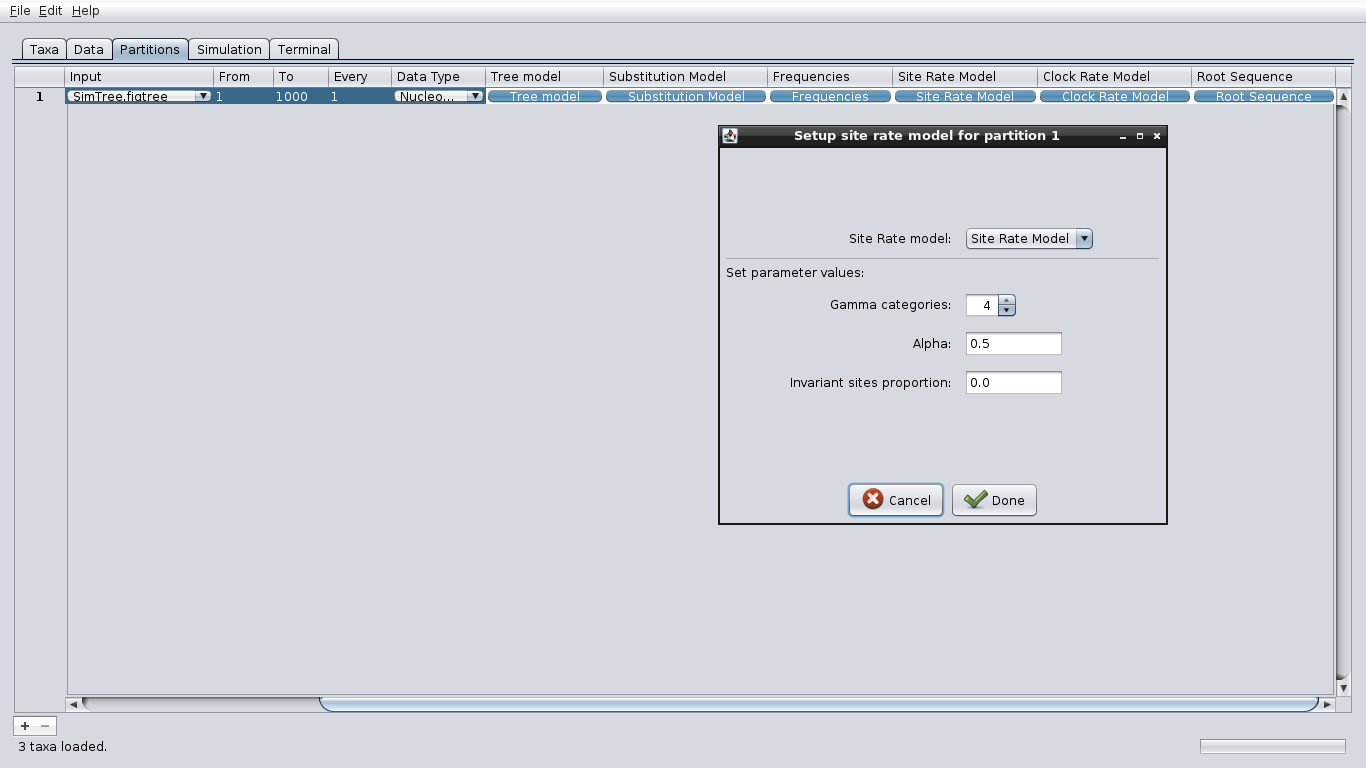
\includegraphics[scale=\figurescale]{GAMMA.png} 
\caption{
{ \footnotesize 
{\bf Site rate heterogeinity.}
Site heterogeinity can be simulated by going to the \textbf{Partitions} and click on the `Site Rate Model' button.
} % END: footnotesize
}
\label{fig:gamma}
\end{figure}
%%

The frequency with which each character (nucleotide or codon) appears is also an important aspect as different organisms may have different base frequencies. 
In {\bussname}, one can specify frequencies for nucleotides or codons by going to the \textbf{Partitions} and click the `Frequency Model' button and specify the frequencies (Figure~\ref{fig:bases}). For nucleotides, four parameters need to be specified (default is $1/4$ for all) and for codons, there are $61$ frequencies to be set -- with $1/61$ uniformly for all as default.

%%
\begin{figure}[h!]
\centering
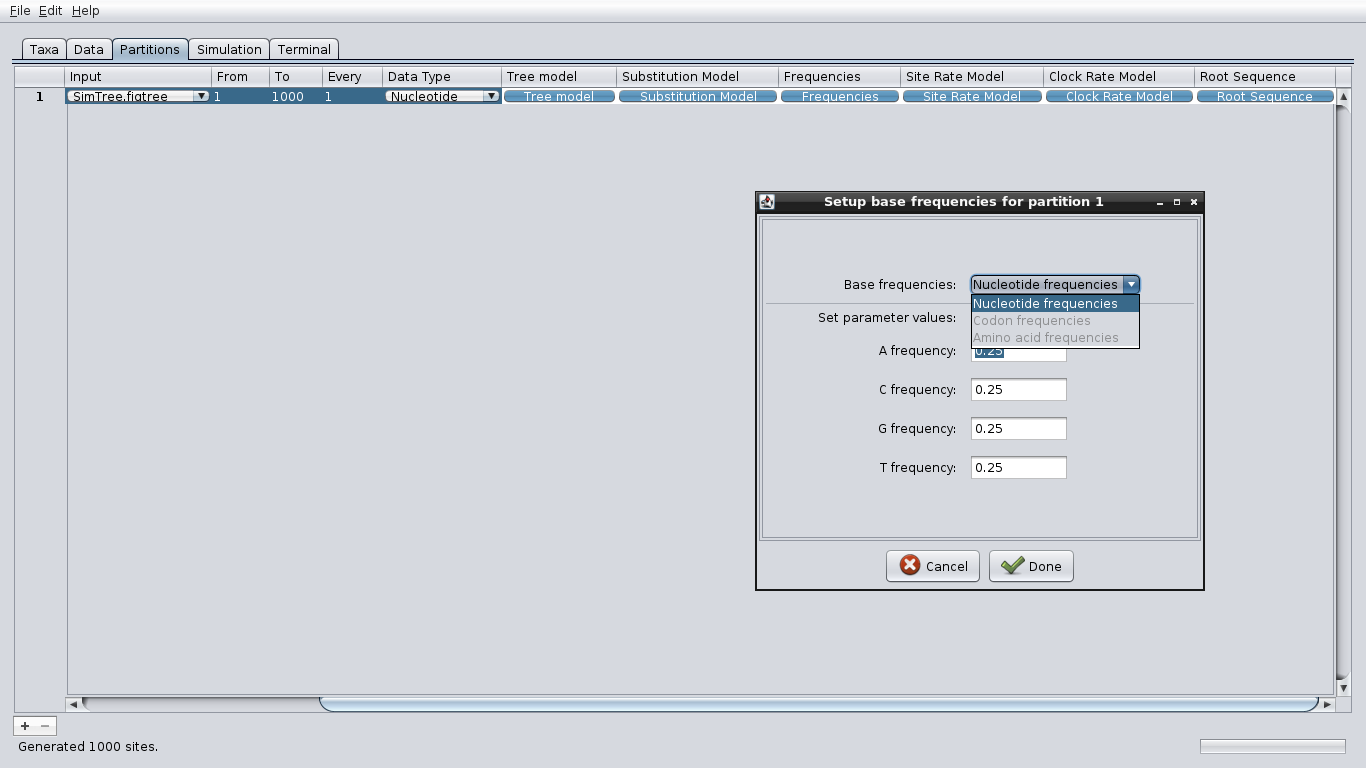
\includegraphics[scale=\figurescale]{BASE_FREQUENCIES.png} 
\caption{
{ \footnotesize 
{\bf Base frequencies.}
To specify base frequencies, go to the \textbf{Partitions} table and click the `Frequency Model' button.
} % END: footnotesize
}
\label{fig:bases}
\end{figure}
%%

\subsection{Molecular clock}

Traditionally, it was assumed that each branch in a phylogeny had the same rate of evolution. 
Numerous studies have shown this assumption not to hold in a number of real-world situations. 
{\bussname} offers several options of relaxed molecular clock models. 
Each model specifies a distribution from which a mutation rate is drawn for each branch in the phylogeny (tree). 
The user can choose between the (default) Strict clock model, as well as three relaxed clock models: Exponential, Log-normal and Inverse Gaussian. 
Each of the relaxed models specifies a distribution with different parameters. 
For the Strict model, the user needs to supply a single parameter, the clock rate. 
For the Exponential model, the mean and offset of the exponential distribution are necessary. 
For Log-normal and Inverse Gaussian models, the user needs to specify mean, standard deviation and offset. 
See Figure \ref{fig:clock2} for an examples.  

%%
\begin{figure}[h!]
\centering
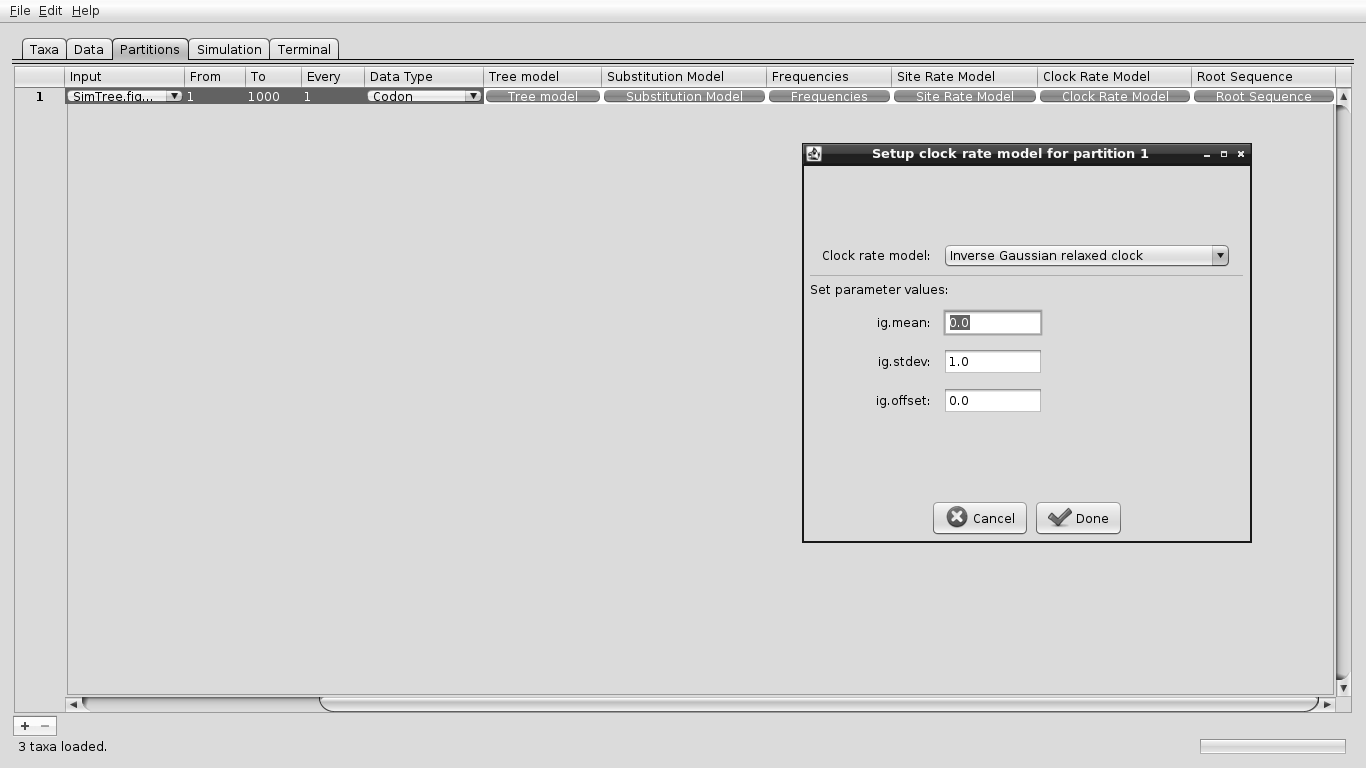
\includegraphics[scale=\figurescale]{CLOCK2.png} 
\caption{
{ \footnotesize 
{\bf Clock model.}
Setting up an Inverse Gaussian relaxed clock with mean$=0$, standard deviation of $1.0$ and no offset.
} % END: footnotesize
}
\label{fig:clock2}
\end{figure}
%%

\subsection{Setting multiple partitions}

Simulating partitions is a way of reproducing the heterogeneity in evolutionary dynamics we observe in different portions of the genome. Every step described above can be repeated for any number of partitions. 
{\bussname} provides an intuitive way of setting multiple partitions, which can have different models and parameters for sequence evolution, site heterogeinity, base frequencies and molecular clock.
% TODO: LM: the role of the 'every' parameter... 
Each partition can either have its own topology, or the tree structure can be shared between partitions.
Partition settings apply from position in the alignment specified as`from' to position specified as `to', on every position being the multiple of `every' parameter.

%%
\begin{figure}[h!]
\centering
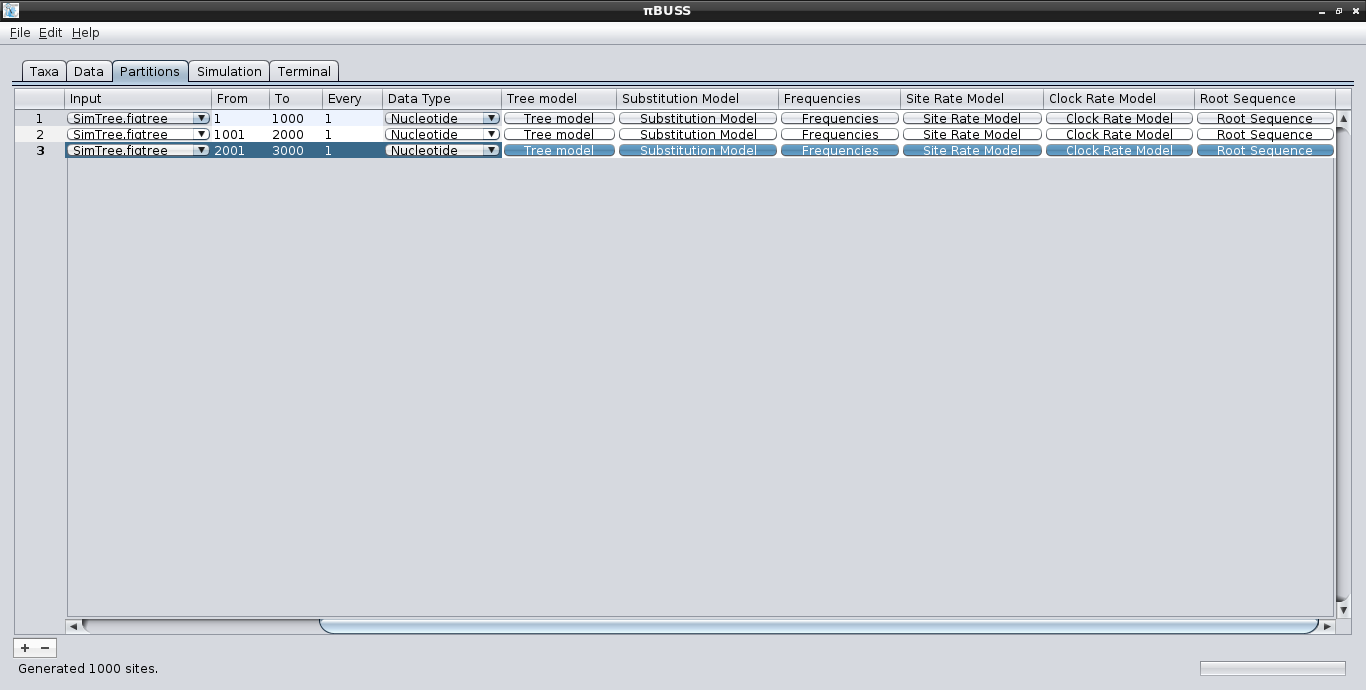
\includegraphics[scale=\figurescale]{MULTIPLE_PARTITIONS.png} 
\caption{
{ \footnotesize 
{\bf Setting multiple partitions.}
You can set up any number of partitions, each with its own tree topology, model of evolution, molecular clock and base frequency. 
Just click the `+' button at the bottom left corner of the GUI window at the \textbf{Partitions} tab.
} % END: footnotesize
}
\label{fig:partitions}
\end{figure}
%%

\subsection{Saving and loading created settings}
Software comes with a simple save/load option, that allows to preserve settings generated via GUI to be loaded or edited at some other time. To store GUI settings go to main menus File and select `Save setting...' to choose name and location for the serialized inputs. 
To load such preserved settings, again choose File $\longrightarrow$ `Load setting...' and navigate to the previous location.

\subsection{Creating and running an XML file}

{\bussname} provides an XML parser that allows the user to store the simulation settings in XML files, that can be later imported into the program and modified if necessary. Importantly, the generated XMLs can be run in BEAST, invoking the core implementation of the simulator.
Another advantage of the XML functionality is that the user can generate XMLs using the GUI and then edit these files to attain more advanced options for data evolving under complex evolutionary scenarios, e.g. an epoch model (see the \textbf{Do the evolution, baby!} section below).
This adds substantial flexibility to users whose needs exceed the complexity of evolutionary scenarios available through the GUI.
XML editing can also be used to simulate discrete phylogeographic trait data (see \textbf{Do the evolution, baby!} for an example) .
To export an XML, just click the `Generate XML' button at the \textbf{Simulation} tab.
To run the generated file, the user just needs to load it into BEAST with BEAGLE. For Windows users, this reduces to double-clicking the BEAST executable and then checking the 'Use BEAGLE library' box. For UNIX/Linux users, issuing 

% LM: Mac users can do something too, which I don't know what is :) Since Mac X is now UNIX, maybe it's the same...
% TODO: review this 'BEAGLE_PATH' stuff
\begin{code}
java -Djava.library.path=\$BEAGLE\_PATH -jar beast.jar -beagle path/to/file.xml
\end{code}

\noindent
at the terminal does the job.
For further details on BEAST/BEAGLE usage, please see \url{http://beast.bio.ed.ac.uk/}.


\subsection{Using the command line interface (CLI)}

{\bussname} offers a command line interface (CLI), that can be used for pipelining in big simulation studies to generate large amounts of different simulation settings.
The CLI options mirror those available from the GUI, with an intuitive syntax.
In table~\ref{tab:commands} we present the CLI options for each feature in {\bussname}.

\begin{table}[h!]
\begin{center}
\tiny{
\begin{tabular}{lcc}
\hline 
\textbf{Parameter} & \textbf{Command} & \textbf{Options}\tabularnewline
\hline 
\cellcolor{snow3}Tree topology & \cellcolor{snow3}-treeFile & \cellcolor{snow3}-\tabularnewline
\hline 
Taxa set & -taxaSet & -\tabularnewline
\hline 
\cellcolor{snow3} & \cellcolor{snow3} & \cellcolor{snow3}-constantPopulationParameterValues\tabularnewline
\cellcolor{snow3} & \cellcolor{snow3} & \cellcolor{snow3}-exponentialGrowthRateParameterValues\tabularnewline
\cellcolor{snow3}\multirow{-3}{*}{Demographic (coalescent) model} & \cellcolor{snow3}\multirow{-3}{*}{-demographicModel} & \cellcolor{snow3}-exponentialDoublingTimeParameterValues\tabularnewline
\hline 
 &  & -HKYsubstitutionParameterValues\tabularnewline
 &  & -GTRsubstitutionParameterValues\tabularnewline
 &  & -TN93substitutionParameterValues\tabularnewline
\multirow{-4}{*}{Markov model of evolution} & \multirow{-4}{*}{-branchSubstitutionModel} & -GY94substitutionParameterValues\tabularnewline
\hline 
\cellcolor{snow3}Site rate heterogeinity & \cellcolor{snow3}-siteRateModel & \cellcolor{snow3}-gammaSiteRateModelParameterValues\tabularnewline
\hline 
 &  & -strictClockParameterValues\tabularnewline
 &  & -lognormalRelaxedClockParameterValues\tabularnewline
 &  & -exponentialRelaxedClockParameterValues\tabularnewline
\multirow{-4}{*}{Molecular clock model} & \multirow{-4}{*}{-clockRateModel} & -inverseGaussianRelaxedClockParameterValues\tabularnewline
\hline 
\cellcolor{snow3} & \cellcolor{snow3} & \cellcolor{snow3}-nucleotideFrequencyParameterValues\tabularnewline
\cellcolor{snow3}\multirow{-2}{*}{Base frequencies} & \cellcolor{snow3}\multirow{-2}{*}{-baseFrequencies} & \cellcolor{snow3}-codonFrequencyParameterValues\tabularnewline
\hline 
Root sequence & -rootSequence & -\tabularnewline
\end{tabular}
} % END: footnotesize
\caption{
{ \footnotesize 
{\bf List of command line options for {\bussname}.}
} % END: footnotesize
}
\label{tab:commands}
\end{center}
\end{table}

As a general example, consider simulating some data under a HKY model, for two partitions of 500 sites each and separate topologies.
The commands for this would look like:

\begin{code}
java -Djava.library.path=\$BEAGLE\_PATH -jar buss.jar -treeFile Tree1.tree -from 1 -to 500 -every 1 -branchSubstitutionModel HKY -HKYsubstitutionParameterValues 1.0 : -treeFile Tree2.tree -from 501 -to 1000-every 1 -branchSubstitutionModel HKY -HKYsubstitutionParameterValues 10.0 : sequences.fasta
\end{code}

Check the \textbf{Do the evolution, baby!} section for more examples of how to use the CLI.

\section{Examples: Do the evolution, baby!}

In this section we present a couple of possible simulations that can be done using {\bussname}.
{\bussname} can either directly generate the data or export the settings to an XML file to be run in BEAST, invoking the core implementation of the simulator.

% new crap on seed and parallel --I'll close the issue
If you want your simulation results to be exactly reproducible, you can set the seed for the random number generator by checking a tick box at the {\bf Simulation} tab.
Also, if you are simulating directly from {\bussname}, you may also want to use the novel and much faster parallel implementation.
This is easily accomplished by checking the corresponding tick box at the {\bf Simulation} tab.
Figure~\ref{fig:simutab} shows a screenshot where both these options are enabled.

Using the CLI, seed is parsed after parsing all the arguments for partitions.
The user can specify a seed and choose to use the parallel implementation by adding 
\begin{code} % TODO: rather not add it to the table, see if you agree
[<output-file-name>] [<seed>] [<true|false>] [<true|false>]
\end{code}
after the last ``:'' sign dividing the desired partitions.
The first true/false statement allows the ancestral sequences in the inner nodes to  be saved -- also accomplished by checking the corresponding box in the {\bf Simulation} tab.
The last argument corresponds to the use of the parallel implementation, which is false by default. 

%%
\begin{figure}[h!]
\centering
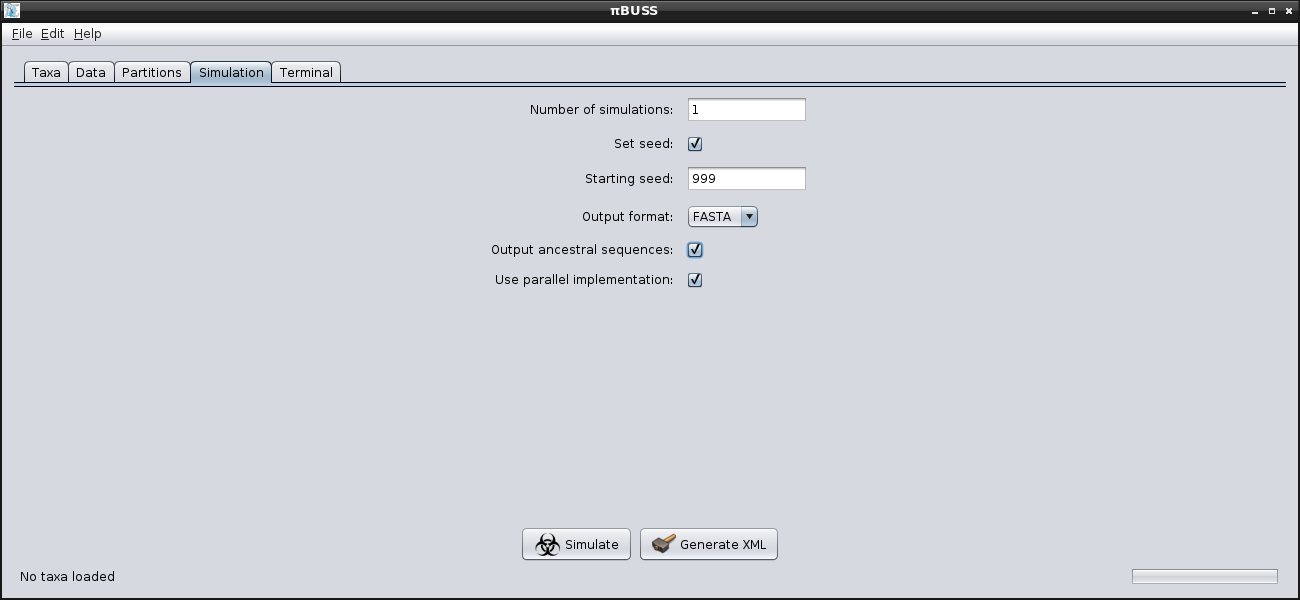
\includegraphics[scale=\figurescale]{SIMUTAB.png} 
\caption{
{ \footnotesize 
{\bf Setting RNG seed.}
To set the seed for your simulation and choose the parallel BEAGLE implementation, check the corresponding tick boxes at the {\bf Simulation} tab.
} % END: footnotesize
}
\label{fig:simutab}
\end{figure}
%%

\subsection{Generating data evolving under GY94 codon model}

To generate sequence data evolving according to codon substitution model we start by importing a backbone tree topology. 
Load the \href{http://rega.kuleuven.be/cev/ecv/software/buss_files/simtree.figtree}{\emph{SimTree.figtree}} tree file shipped with this tutorial as described in \emph{\loading} subsection.   

Then move to \textbf{Partitions} panel and select the just loaded topology from the drop-down list in the \emph{Data} column. 
Next click on the button under the \emph{Base Frequencies} column, select codon frequencies as shown in the Figure \ref{fig:CodonFrequencies}.
Confirm your choice and move to \textbf{Simulation} panel to generate XML or simulate a fasta or nexus file.

\begin{figure}[h!]
\centering
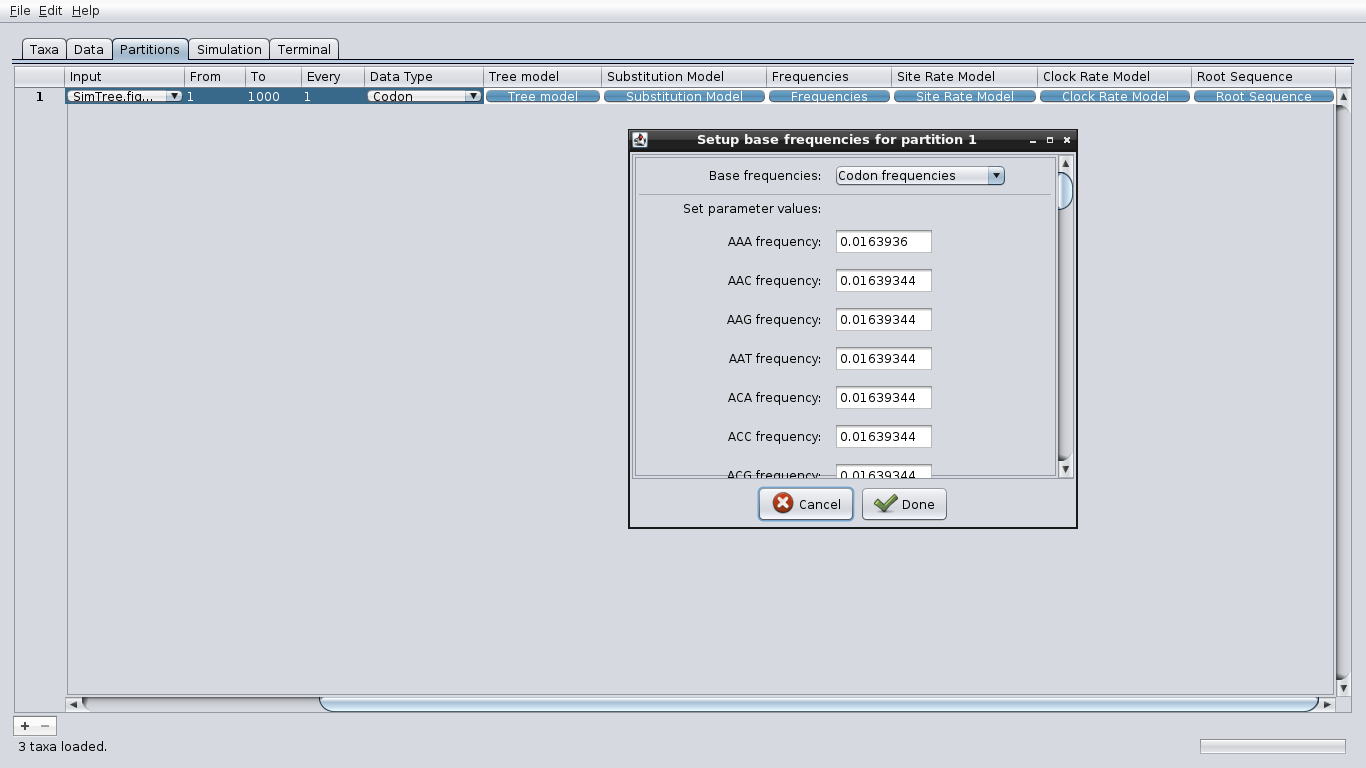
\includegraphics[scale=\figurescale]{CODON_FREQUENCIES.png} 
\caption{
{ \footnotesize 
{\bf Setting codon frequencies.}
Just select codon frequencies in the drop-down menu and you're done. The default is $1/61$ for each codon.
} % END: footnotesize
}
\label{fig:CodonFrequencies}
\end{figure}

\subsection{Generating codon partitioned data}
As before start by loading the \href{http://rega.kuleuven.be/cev/ecv/software/buss_files/simtree.figtree}{\emph{SimTree.figtree}} tree file, this time we will however need to set three separate partitions, from different positions in the alignment and simulating to every third alignment position, just like in Figure \ref{fig:CodonPartitoning}.

\begin{figure}[h!]
\centering
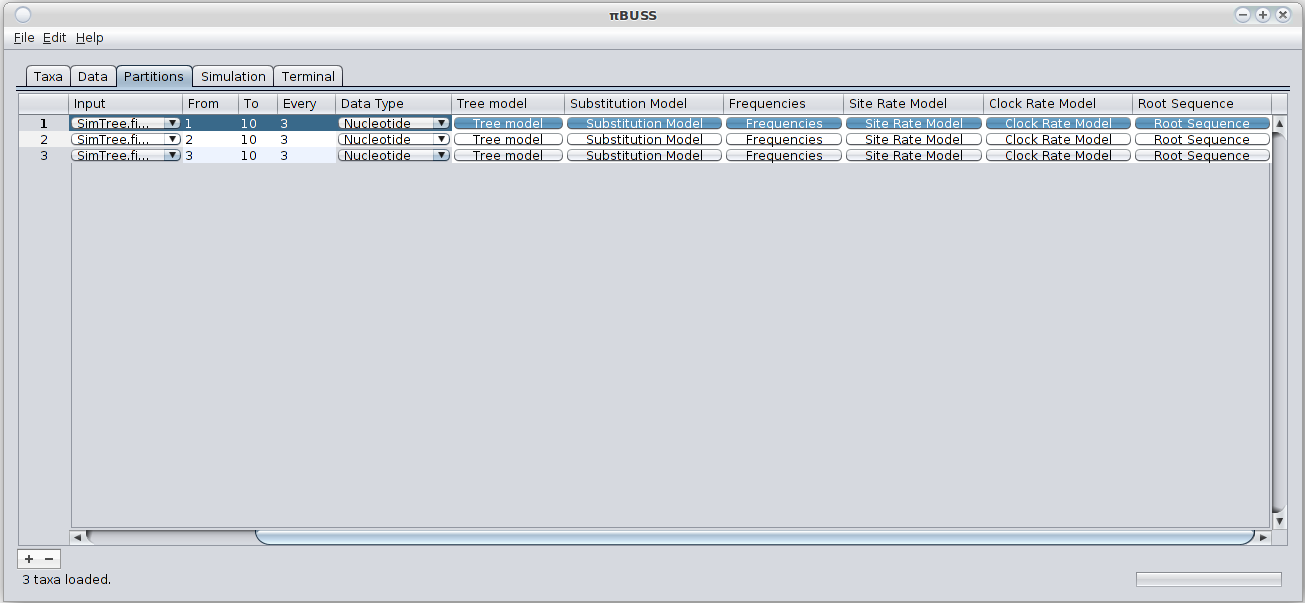
\includegraphics[scale=\figurescale]{CODON_PARTITIONING.png} 
\caption{
{ \footnotesize 
{\bf Codon partitioned simulation.}
} % END: footnotesize
}
\label{fig:CodonPartitoning}
\end{figure}

We can change the substitution dynamics under which the data will be generated by modifying the default value of the HKY model $\kappa$ parameter, for example for the second partition.
Change the $\kappa$ parameter value to $10.0$ using \emph{Branch Substitution Model} button in the second row of the \textbf{Partitions} panel and go to \textbf{Simulation} panel to generate the output.

Equivalently one might use the CLI interface, then the above operations sum up to issuing the following command:

\begin{code}
java -Djava.library.path=/usr/local/lib -jar buss.jar 
-treeFile SimTree.figtree.tree -from 1 -to 1000 -every 3 -branchSubstitutionModel HKY -branchSubstitutionModel HKY -HKYsubstitutionParameterValues 1.0 :
-treeFile SimTree.figtree.tree -from 2 -to 1000 -every 3 -branchSubstitutionModel HKY -branchSubstitutionModel HKY -HKYsubstitutionParameterValues 10.0 :
-treeFile SimTree.figtree.tree -from 3 -to 1000 -every 3 -branchSubstitutionModel HKY -branchSubstitutionModel HKY -HKYsubstitutionParameterValues 1.0 :
sequences.fasta
\end{code}

\subsection{Simulating a tree topology}
{\bussname} can be used to simulate a bifurcating tree topology under the coalescent process driven by a specified model. 
The only input needed in this case is a set of taxa with corresponding heights. 
These can be loaded from an existing tree topology or specified using the editor in \textbf{Data} panel, under \emph{Taxa set} column.

In this example we will use a set of taxa shipped with this tutorial in \href{http://rega.kuleuven.be/cev/ecv/software/buss_files/taxa.txt}{\emph{taxa.txt}} file. Use the editor's \emph{Load} button to import the file like in Figure \ref{fig:TaxaEditor}.

Set the taxa as simulations backbone in drop-list under \emph{Data} column in \textbf{Partitions} panel.

\begin{figure}[h!]
\centering
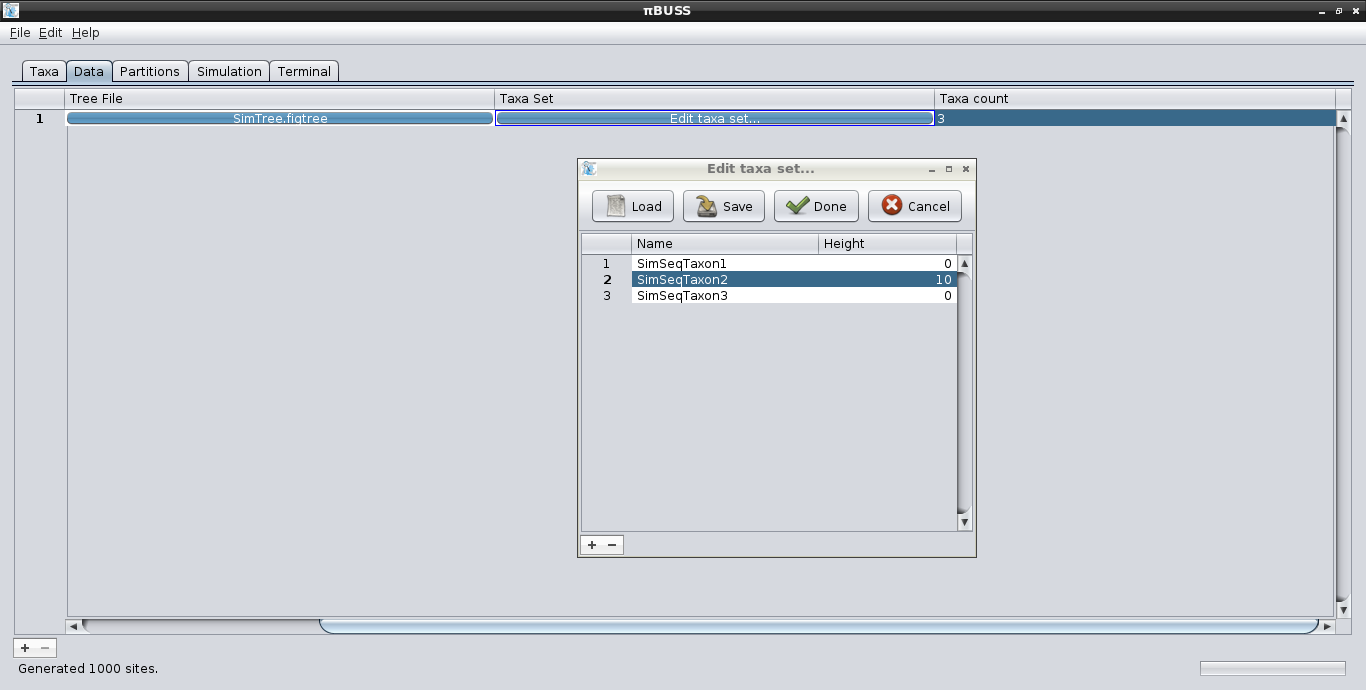
\includegraphics[scale=\figurescale]{TAXA_EDITOR.png} 
\caption{
{ \footnotesize 
{\bf Loading a taxa set from tab-separated file.}
Once you load the taxa set onto {\bussname}, you are ready to simulate under any of the coalescent dynamics available.
} % END: footnotesize
}
\label{fig:TaxaEditor}
\end{figure}   

Now it's time to set the demographic model that will drive the coalescent. Click on the editor button under \emph{demographic model} column and choose the \emph{Constant Population} model with \emph{Population Size} parameter of $50.0$, like shown in Figure \ref{fig:DemoModel} below.

\begin{figure}[h!]
\centering
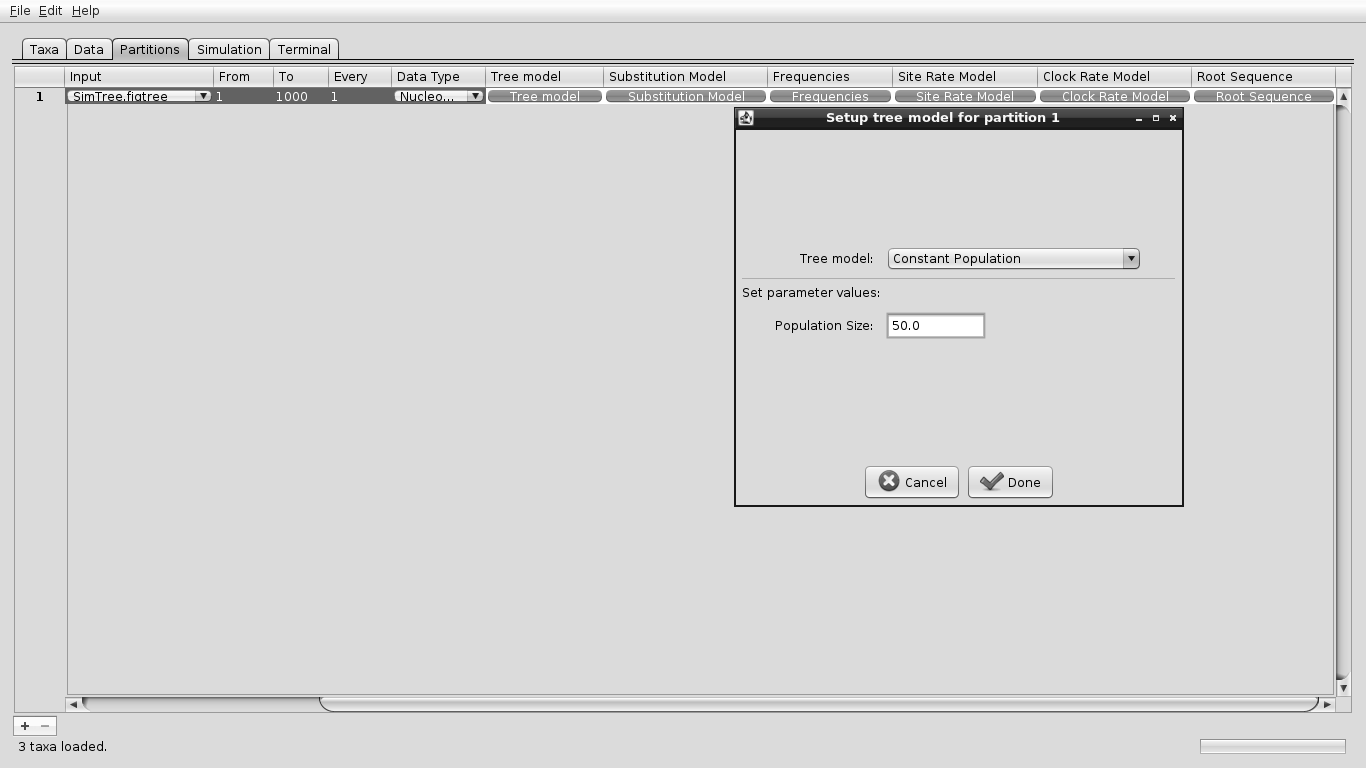
\includegraphics[scale=\figurescale]{DEMOGRAPHIC_MODEL.png} 
\caption{
{ \footnotesize 
{\bf Loading a taxa set from tab-separated file.}
} % END: footnotesize
}
\label{fig:DemoModel}
\end{figure}  

To generate the data, click on the \emph{Simulate} button in the \textbf{Simulation} panel. The generated tree (newick format) can be copy-pasted from \textbf{Terminal} panel as shown in Figure \ref{fig:Terminal}.

\begin{figure}[h!]
\centering
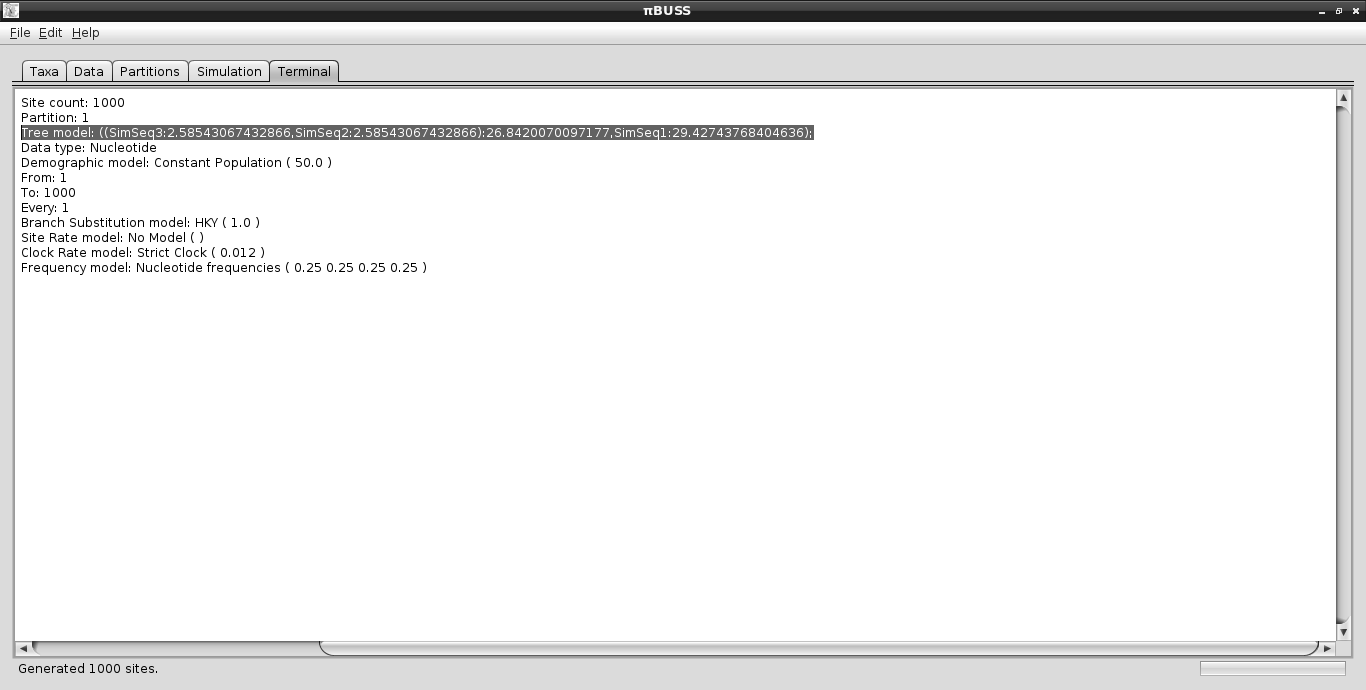
\includegraphics[scale=\figurescale]{TERMINAL_OUTPUT.png} 
\caption{
{ \footnotesize 
{\bf Terminal output.}
} % END: footnotesize
}
\label{fig:Terminal}
\end{figure} 

\subsection{Extending a created XML to generate discrete phylogeographical trait data}
By modelling  phylogeography as a continuous-time Markov chain (CTMC) we are able to make use of the same computational machinery used for the branch substitution Markov models. In this setting, each location is treated as a state of the chain and we can set transition/transversion parameters in the same fashion.

In addition to command-line and graphical interface, {\bussname} is capable of producing XML files that can be used with BEAST software to invoke the core implementation of the software. 
For large and complex simulation studies this should be the preferred way of interacting with the software.

We can use the default XML generated for us by {\bussname} as a canvas to extend to discrete geographical trait simulation. 
Start with loading the \href{http://rega.kuleuven.be/cev/ecv/software/buss_files/simtree.figtree}{\emph{SimTree.figtree}} tree file and setting it as data in \textbf{Partitions} panel. 
Now go to the \textbf{Simulation} panel and click on \emph{Generate XML} button, saving the file as \emph{generate\_sequences.xml}.
Open the generated file in your favourite text editor.

We need to define the discrete geographical locations that {\bussname} will sample from. After the  {\color{darkblue}taxa} block paste the following code:

\begin{lstlisting}
<generalDataType id="geography"> 
  <state code="location1"/>
  <state code="location2"/>
  <state code="location3"/>
</generalDataType>
\end{lstlisting}

Scroll to the {\color{darkblue}frequencyModel} block. Because we have specified $K=3$ discrete locations we need to specify base frequencies for them. Delete the existing {\color{darkblue}frequencyModel} block and paste there following code instead:

\begin{lstlisting}
<frequencyModel id="freqModel">
  <generalDataType idref="geography"/>
    <frequencies>
      <parameter dimension="3" value="0.3 0.3 0.4"/>
    </frequencies>
</frequencyModel>
\end{lstlisting}

Now scroll further down to the substitution model block (defined between {\color{darkblue}HKYModel} tags if you generated the XML using default settings). 
We need to define a geographical substitution model, driven by a rate matrix. 
We specify $K\times(K-1)=6$ entries such that the underlying instantaneous rate matrix is asymmetric (non-reversible). 
Replace the existing block with: 

\begin{lstlisting}
<complexSubstitutionModel id="originModel.simulation" randomizeIndicator="false">
  <generalDataType idref="geography"/>
  <rootFrequencies>
    <frequencyModel idref="freqModel"/>
  </rootFrequencies>
  <rates>
    <parameter id="rates.simulation" dimension="6" value="1.0"/>
  </rates>
</complexSubstitutionModel>
\end{lstlisting}

Now reference the created substitution model inside {\color{darkblue}siteModel} tags like this:

\begin{lstlisting}
<siteModel id="geoSiteModel.simulation">
  <substitutionModel>
    <complexSubstitutionModel idref="originModel.simulation"/>
  </substitutionModel>
</siteModel>
\end{lstlisting}

Finally all the new elements need to be referenced in the {\color{darkblue}beagleSequenceSimulator} block. We specify one replicate, as every taxa can ultimately have only one geographical trait:

\begin{lstlisting}
<beagleSequenceSimulator id="simulator">
  <partition from="1" to="1"> 
    <treeModel idref="treeModel1"/>
    <complexSubstitutionModel idref="originModel.simulation"/>	    
    <siteModel idref="geoSiteModel.simulation"/>
    <strictClockBranchRates idref="branchRates1"/>
    <frequencyModel idref="freqModel"/>
  </partition>
</beagleSequenceSimulator>
\end{lstlisting}

Resulting document is availiable as \href{http://rega.kuleuven.be/cev/ecv/software/buss_files/generate\_discrete\_phylogeography\_SimTree.xml}{\emph{generate\_discrete\_phylogeography\_SimTree.xml}} file shipped with this tutorial.
The created XML can be invoked within BEAST to generate the trait data by issuing the following command:

\begin{code}
java -Djava.library.path=\$BEAGLE\_PATH -jar beast.jar -beagle\_CPU generate\_sequences.xml
\end{code}

Note that the presented example is just a fraction of analysis possible by editing the \bussname/BEAGLE XMLs and we urge the users to play with the availiable options. 

\section{Final Remarks}

\subsection{License}
% LM: licence info I found at BEAST source 
This is free software; you can redistribute it and/or modify it under the terms of the {GNU} Lesser General Public License as published by the Free Software Foundation; either version 2 of the License, or (at your option) any later version. This software is distributed in the hope that it will be useful, but {WITHOUT ANY WARRANTY}; without even the implied warranty of {MERCHANTABILITY} or {FITNESS FOR A PARTICULAR PURPOSE}. See the ``GNU Lesser General Public License'':\url{http://www.gnu.org/licenses/lgpl.html} for more details.

\subsection{Availability and requirements}
Beagle Sequence Simulator's source code is freely available as a GoogleCode repository:
\url{http://code.google.com/p/beast-mcmc/}
Compiled, runnable packages targeting all major platforms along with tutorial on using the software are hosted at:
\url{http://rega.kuleuven.be/cev/ecv/software/buss}.

\subsection{Citing {\bussname}}
We have invested a lot of time and effort in creating {\bussname}, please cite it when using it in your research. BibTeX entry:

\begin{code}
@Article\{bielejec2014, \\
AUTHOR = \{Bielejec, Filip and Lemey, Philippe and Carvalho, Luiz
and Baele, Guy and Rambaut, Andrew and Suchard, Marc A.\}, \\
TITLE = \{piBUSS: a parallel BEAST/BEAGLE utility for sequence simulation
under complex evolutionary scenarios\}, \\
JOURNAL = \{BMC Bioinformatics\}, \\
VOLUME = \{15\}, \\
YEAR = \{2014\}, \\
NUMBER = \{1\}, \\
PAGES = \{133\} \\
\}
\end{code}
